\chapter*{BIODATA PENULIS}
%*********************************
%Gambar Foto 
	\begin{center}
		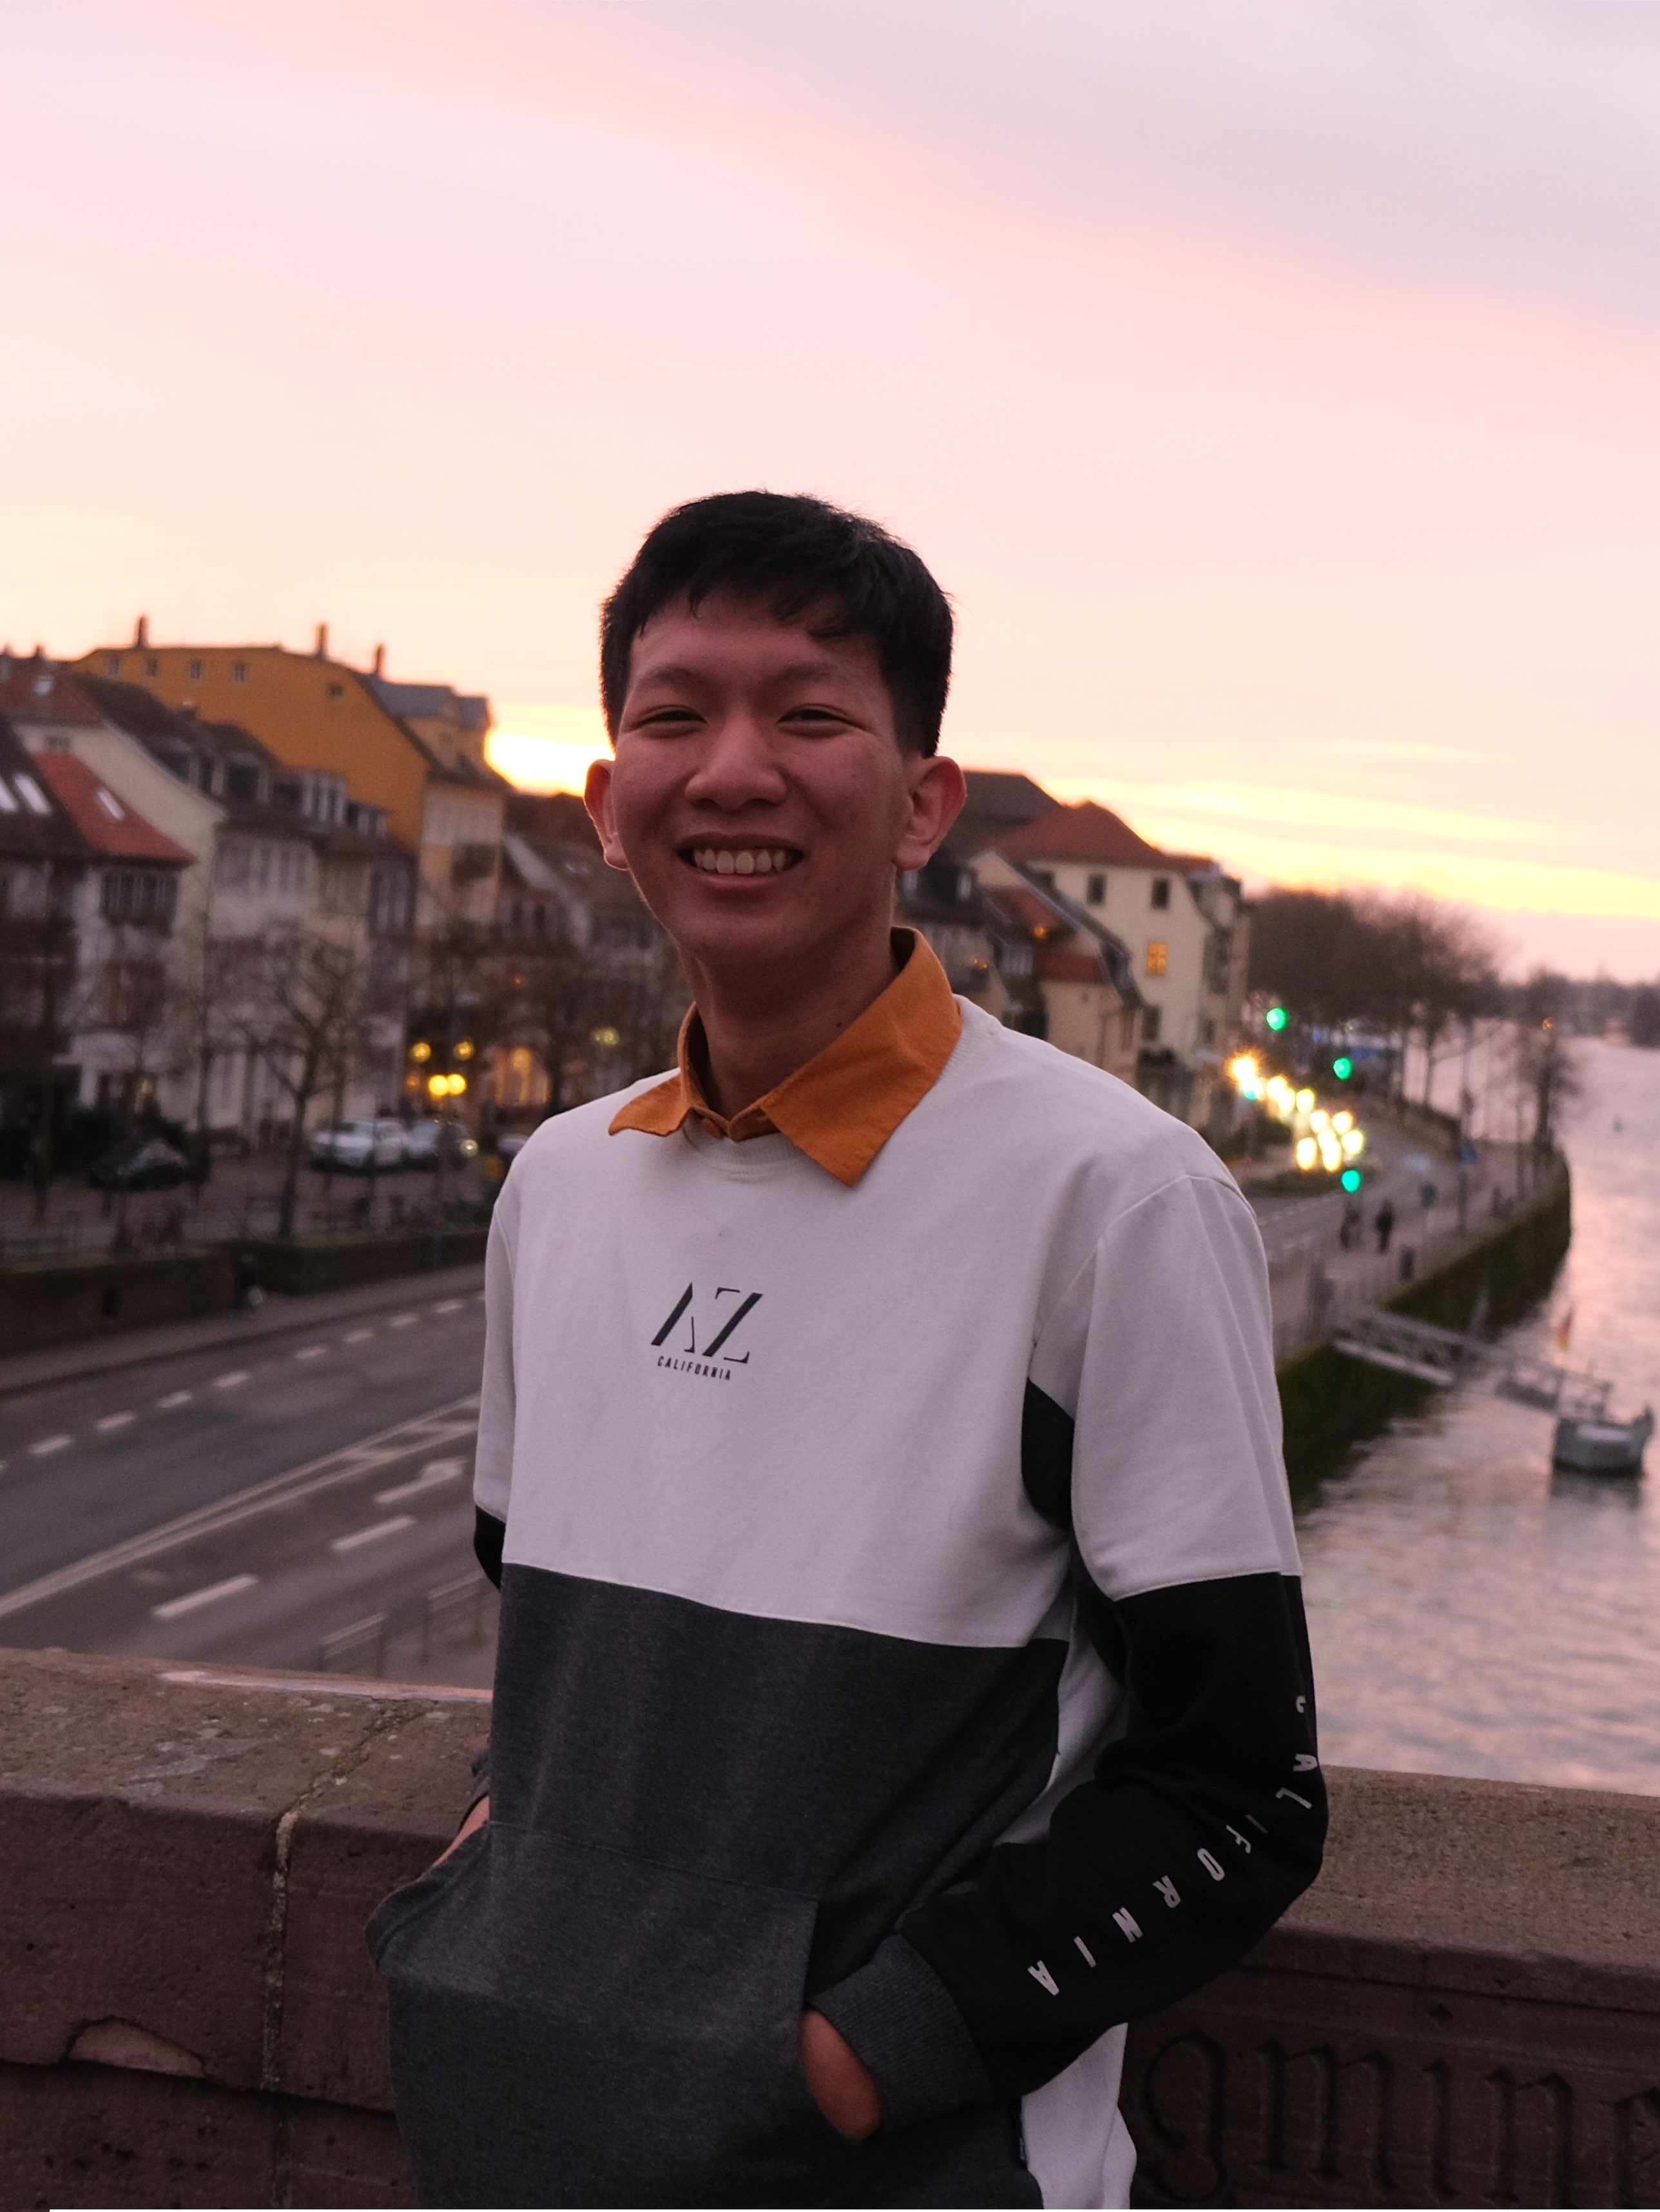
\includegraphics[height=0.2\textheight]{./ubah/Foto}
	\end{center}
%*********************************
\section*{Identitas Diri}
\begin{tabular}{p{3cm}cp{9cm}}
	%Masukan Identitas Disini.............
	Nama  		  & :&
		Lukas Purba Wisesa \\
	Tempat Lahir  & :&
		Rembang\\
	Tanggal Lahir &:& 
		24 November 1999\\
	Alamat        &:& J
		Jalan Diponegoro 28\\
%	Identitas 1   &:&
%		 Isi Identitas 1\\
%	Identitas 2   &:& 
%		Isi Identitas 2\\
%	Identitas 3   &:&
%		 Isi Identitas 3\\
%	Identitas 4   &:&
%		 Isi Identitas 4\\
\end{tabular}

\section*{Riwayat Pendidikan}
\begin{tabular}{p{3cm}cp{9cm}}
	2020-sekarang  & :&
		Program Master (S2), Departemen Teknik  Elektro, Fakultas Teknologi Elektro dan Informatika Cerdas, Institut Teknologi  Sepuluh Nopember\\
	&&\\
	2017-2021  & :&
		Program Sarjana (S1), Departemen Teknik  Elektro, Fakultas Teknologi Elektro dan Informatika Cerdas, Institut Teknologi  Sepuluh Nopember\\
	% &&\\
	% 0000-0000  & :&
	% 	Pendidikan 1\\
	% &&\\
	% 0000-0000  & :&
	% 	Pendidikan 2\\
	% &&\\
	% 0000-0000  & :&
	% 	Pendidikan 3\\
\end{tabular}


% \section*{Daftar Publikasi}

% \begin{enumerate}
% 	\item Setiyoutami, A., Anggraeni, W., Purwitasari, D., Yuniarno, E.M., Purnomo, M.H.,\textit{Extracting Temporal-Based Spatial Features in Imbalanced Data for Predicting Dengue Virus Transmission},
% 	Advances in Intelligent Systems and Computing, 2021, 1158, pp. 731–742
% 	\item Salsabila, F.N., Yuhana, U.L., Yuniarno, E.M., Purnomo, M.H., \textit{Sifte-math, a sifteo based mathematics assessment serious game for deaf children}, IES 2020 - International Electronics Symposium: The Role of Autonomous and Intelligent Systems for Human Life and Comfort, 2020, pp. 620–625, 9231578
	
	
% \end{enumerate}

% \section*{Riwayat Penelitian}
% \begin{enumerate}
% 	\item \lipsum[3]
% 	\item \lipsum[3]
% 	\item Penelitian Ke Tiga 
% 	\item Penelitian Ke Empat 
% \end{enumerate}
\section*{Tentang Penulis}
Lukas Purba Wisesa, merupakan seseorang mahasiswa yang 
berasal dari Institut Teknologi Sepuluh Nopember departemen Teknik Elektro. Penulis merupakan lulusan S1 Institut 
Teknologi Sepuluh Nopember. Dalam masa kuliah, penulis tertarik pada bidang pengembangan \textit{artificial 
intelligence}  dan pembelajaran mesin. Selain itu, penulis juga aktif dalam melakukan analisis sebagai hobi 
dimana pekerjaan penulis dapat diakses di github.com/lukaspurbaw. Penulis juga aktif dalam mengikuti kompetisi 
pengembangan model data science di ajang NDSC 2020. Bagi pembaca yang memiliki kritik, saran, atau pertanyaan 
mengenai laporan thesis ini dapat menghubungi penulis melalui surel lukaspurbaw@gmail.com.